\section{Transliteration with WFST}

% \subsection*{Goal}

% Transliteration is to ``spelling out'' a word in another alphabet, i.e., replace the characters with phonetic approximations, by mapping strings in one set to another set.

\textbf{Def}: Weighted finite-state transducers $T=\langle Q, \Sigma, \Omega, \lambda, \rho, \delta\rangle$ consist of: (1) $Q$ a finite set of states (including initial or ending); (2) $\Sigma$, input vocab; (3) $\Omega$, output vocab; (4) $\lambda$: $Q\to$initial scores; (5) $\rho$: $Q\to$final scores; (6) $\delta$: arc $q_i\to q_j$ to transition scores. If no output vocab, WFST is a WFSA(acceptor).
% Weighted finite-state transducers is a probabilistic model that map strings from input vocabulary to output vocabulary. The number of states of our modeled language is finite, and the transition is weighted. Each transition is labeled by an input character, an output character and a weight. If the transition does not include the output character, then it is a weighted finite-state acceptor.

\subsection*{Probabilistic model for transition sequences}
$\pi$: path that generates the input $X$ and output $Y$, $\score(\pi) = \sum_i \score(\pi_i)$. Assume $p(y\mid x)=\frac{1}{Z} \sum_\pi \exp(\sum_i \score(\pi_i))$. \textbf{Goal}: find the min/max score path.

\subsection*{Floyd-Warshall Algo $O(N^3)$ (semi ring version)}
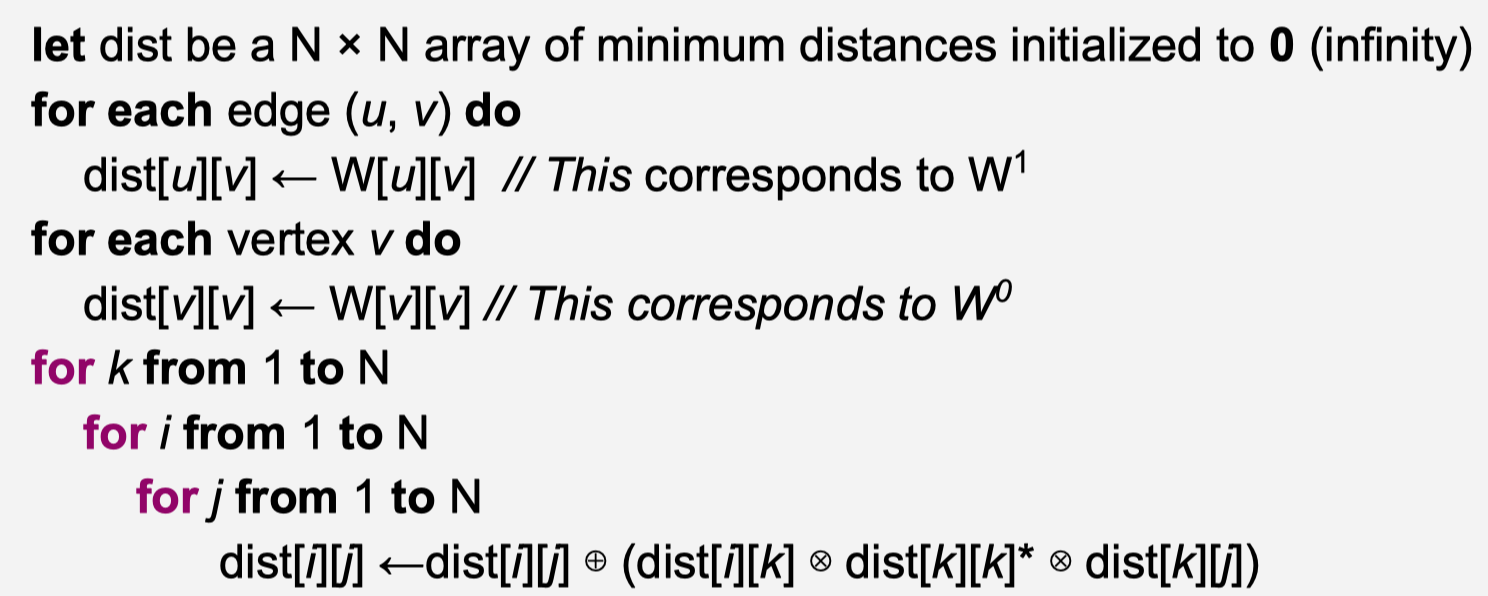
\includegraphics[width=\columnwidth]{img/FWalgoSemiRing.png}
\textbf{Shortest Path}: Real semiring. \textbf{Partition function $\mathcal{Z}$}: Inside semiring.

\subsection*{Kleene's Star $r^{*}$}
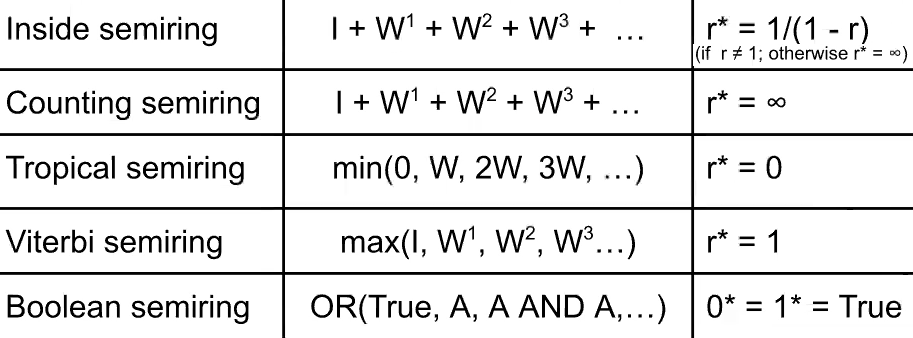
\includegraphics[width=\columnwidth]{img/KleeneStar.png}

\subsection*{Normalizer computation}

$\mathbb{\alpha}$: starting weight; $\mathbb{\beta}$ ending weights; $W^{\omega}$ weight matrix for arc $\omega$. Partitoin function $Z = \alpha^T (\sum_{\omega\in \Omega\cup \{\epsilon\}} W^{\omega})^* \beta$, where the $*$ (Kleene closure) is computed by FW algo with Inside semiring.

